\documentclass{beamer}
\usefonttheme[onlymath]{serif}
\setbeamerfont{footnote}{size=\tiny}
\usetheme{Boadilla}
% enable to get point-by-point reveals
%\beamerdefaultoverlayspecification{<+->}
\usepackage{amsmath}
\usepackage{amssymb}
\usepackage[backend=bibtex]{biblatex}
%\usepackage[multiple]{footmisc}
\usepackage{color}
\usepackage{comment}
\usepackage{datetime}

\usepackage{tikz}
\usepackage{pgffor}
\usetikzlibrary{arrows,positioning}

\usepackage{graphicx}
\graphicspath{{figures/}}

\newdateformat{monthyear}{\monthname[\THEMONTH] \THEYEAR}

\newcommand{\subitem}[1]{\begin{itemize} \item #1 \end{itemize}}

\setbeamertemplate{caption}{\raggedright\insertcaption\par}

% My commands
\newcommand{\R}{\mathbb{R}}
\newcommand{\E}{\mathbb{E}}
\newcommand{\TODO}[1]{\textcolor{red}{\textbf{TODO: #1}}}
%\newcommand{\TODO}[1]{}

\newcommand{\cA}{\mathcal{A}}
\newcommand{\cD}{\mathcal{D}}
\newcommand{\cH}{\mathcal{H}}
\newcommand{\cL}{\mathcal{L}}
\newcommand{\cN}{\mathcal{N}}
\newcommand{\cO}{\mathcal{O}}
\newcommand{\cS}{\mathcal{S}}
\DeclareMathOperator*{\argmax}{argmax}

\newcommand{\sysid}{dynamics}
\newcommand{\blind}{\emph{blind}}
\newcommand{\plain}{\emph{plain}}
\newcommand{\extra}{\emph{extra}}
\newcommand{\embed}{\emph{E2ID}}
\newcommand{\traj}{\emph{traj}}
\newcommand{\embedfn}{e}
\newcommand{\idfn}{{id}}
\newcommand{\latent}{\cL}

\newcommand{\good}[1]{\textcolor{blue}{#1}}
\newcommand{\bad}[1]{\textcolor{red}{#1}}

\bibliography{bibliography}{}


\title[Embed to Identify]{Embed to Identify: Learning an Abstract \\
System Identification Space for Adaptive Control\\ with Deep Reinforcement Learning}
\author[James A. Preiss et al.]{James A. Preiss, Karol Hausman, Gaurav S. Sukhatme}
\institute[USC]{University of Southern California}
\date{\monthyear\today}

% make a section name only slide for each section.
\AtBeginSection[]{
	\begin{frame}
	\vspace{1cm}

	{\centering \Huge \insertsectionhead\par}%

	\end{frame}
}


\begin{document}
\frame{\titlepage}


\begin{frame}
\frametitle{Problem Statement}
Simulation to Reality transfer for robotics is difficult.

\begin{itemize}
\item Successes often rely on engineered high-level action spaces that are far from, e.g., motor voltages~\footfullcite{OpenAI-dexterous}$^,$\footfullcite{kaufmann-learning-agile-flight}

\item Limitations of low-level control middleware may prevent fully exploiting physical abilities of system
\item Rather than abstracting physics, we want policies that can adapt to uncertain physics online
\end{itemize}
\end{frame}

\section{Related Work}

\begin{frame}
\frametitle{Related work: Domain randomization}
\emph{Domain Randomization} in visual~\footfullcite{tobin-domainrand-arxiv17}
and dynamics simulations has shown good results,
but only when the simulations are small perturbations around reality.
\begin{center}
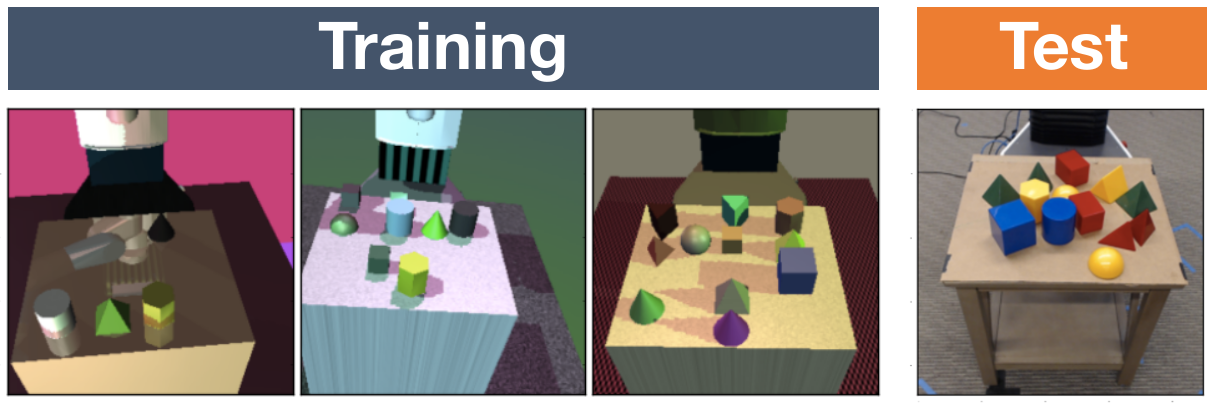
\includegraphics[width=0.75\textwidth]{tobin-visual-domain-randomization.png}

{\footnotesize Image from Tobin et al., 2017}
\end{center}
\textbf{Issues:}
As we will show, it is not enough when the optimal policy differs substantially across the set of possible systems.
\end{frame}

\begin{frame}
\frametitle{Related work: Few-shot methods}
\textbf{Idea:} robot gets a short amount of time to learn from the test environment before it's required to perform optimally.

\begin{block}{\emph{Model-Agnostic Meta-Learning} (Chelsea Finn et al.)}
\begin{columns}
\column{0.55\linewidth}
Optimize for policy parameters that can adapt to the environment in a single step of gradient descent.
\column{0.36\linewidth}
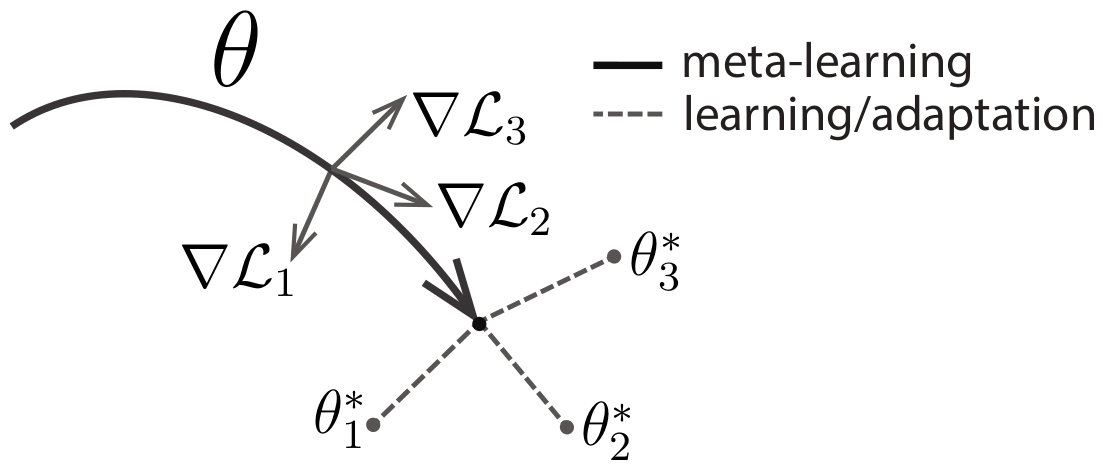
\includegraphics[width=\columnwidth]{maml.png}
\end{columns}
\end{block}
\begin{block}{\emph{RL$^2$} (Yan Duan et al.)}
Train a recurrent policy with persistent internal state,
such that information about the test environment can be stored across episodes.
\end{block}
\textbf{Issues:}
no incentive for good performance when first deployed in test enviornment,
before information is gathered.
\end{frame}

\begin{frame}
\frametitle{Related work: Matched pair methods}
\textbf{Idea:} learn a mapping between the training environment
and exactly one test environment, with limited information about the latter.

\begin{block}{\emph{Mutual Alignment Transfer Learning} (Markus Wulfmeier et al.)}
\begin{columns}
\column{0.61\linewidth}
Train an RL policy in each environment.
Discriminator tries to tell state distributions apart.
Policies rewarded for visiting states that confuse the discriminator.
\column{0.35\linewidth}
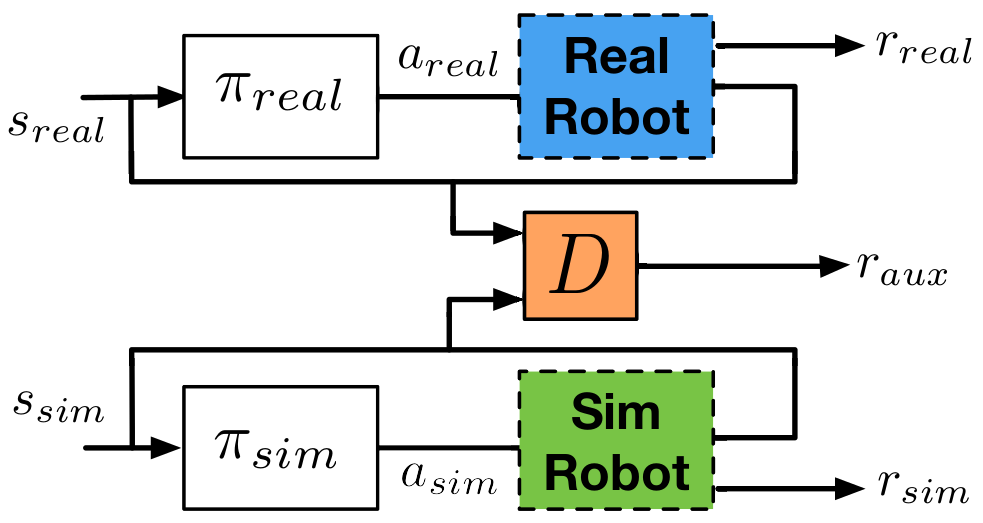
\includegraphics[width=\columnwidth]{mutual-alignment.png}
\end{columns}
\end{block}

\begin{block}{\emph{GeneSIS-RT} (Gregory J. Stein and Nicholas Roy)}
\begin{columns}
\column{0.56\linewidth}
CycleGAN converts game engine images into realistic images.
Ground truth labels, etc. from simulation provides abundant data for supervised learning.
\column{0.4\linewidth}
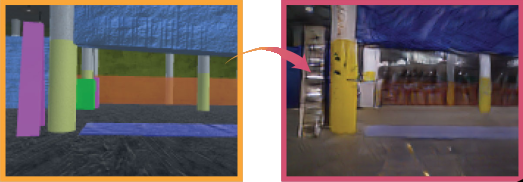
\includegraphics[width=\columnwidth]{genesis-rt.png}
\end{columns}
\end{block}
\textbf{Issues:}
Difficult to scale up to a larger set of test environments.
\end{frame}

\section{Our Approach}

\begin{frame}
\frametitle{Near miss}
\begin{center}
{\Large ``Near miss''} \\
\emph{Learning a Universal Policy with Online System Identification} \\
Wenhao Yu et al., RSS 2017
\begin{alignat*}{2}
\text{policy}\ &: \pi(a|s,d) & & : \cS \times \cD \mapsto \R_{\geq 0} \\% \text{where}\ \mu = \text{dynamics parameters}
\text{SysID}\ &: \phi(s_{[-K:]}, a_{[-K:]}) & & : (\cS \times \cA)^K \mapsto \cD
\end{alignat*}
where $\cS = \text{states},\ \cA = \text{actions},\ \cD = \text{dynamics parameters}.$
\end{center}

\end{frame}

\begin{frame}
\frametitle{Learning an abstract embedding space for SysID}
\centering
\good{\Large Key idea:}

Identifying the true dynamics parameters is \bad{more work} than necessary.

We only need to capture enough information about the environment

for the policy to adapt its behavior correctly.

\vspace{0.7cm}
\good{\Large Response:}

While training the policy, simultaneously learn a mapping
from $\cD$ to an \good{embedding space} $\cL$
that is both \good{easy to identify} and
\good{sufficient for good policy performance}.

\end{frame}

\begin{frame}
\frametitle{E2ID framework}
\centering
\scalebox{0.85}{
\begin{minipage}{\textwidth}
\textbf{Training Time:}

\vspace{0.4cm}
\begin{tikzpicture}[scale=0.8, every node/.style={scale=0.85}]
\tikzstyle{box}=[draw=black, fill=white, inner sep=2mm, rounded corners=1mm]
\tikzstyle{bigbox}=[box, minimum height=1.6cm]
\tikzstyle{branch}=[circle,inner sep=0pt, minimum size=0.15cm, fill=black]
\tikzstyle{arrow}=[->]

\node[bigbox, align=center] (enviro) {Simulation \\ Environment};
\node[bigbox, align=center, right=1.75cm of enviro] (policy) {Policy \\ $\pi$};
\node[box, below=of enviro.south east, xshift=0.3cm] (embedder) {Embedder $\embedfn$};
\node[box, right=of policy, align=center] (traj)
{
  Trajectory $\tau$ \\
  \begin{tikzpicture}
  \foreach \offset in {1,...,5}
  {
    \node[box, sharp corners] (\offset) at (-0.05 * \offset, 0.1 * \offset) {$s_{t - 1},\ a_{t-1}$};
  }
  \end{tikzpicture}
};
\node[box, right=of traj] (estimator) {Estimator $\idfn$};
\node[box, below=0.65cm of traj, align=center] (sup-loss) {Supervised\\ Learning Loss};

\draw [arrow] ([yshift=0.4cm]enviro.east) -- node [above] {states} ([yshift=0.4cm]policy.west);
\draw [arrow] ([yshift=-0.4cm]policy.west) -- node [below] {actions} ([yshift=-0.4cm]enviro.east);
\draw [arrow] ([xshift=-0.5cm]enviro.south) |- node [pos=0.25, right] {SysID} (embedder.west);
\draw [arrow] (embedder.east) -| node [branch, label=below:{embeddings}] (embeds) {} (policy.south);
\draw [arrow] (traj) -- (estimator);
\draw [arrow] ([xshift=0.5cm]estimator.south) |- node [pos=0.35, left, align=right] {estimated\\embeddings} (embeds-|sup-loss.east);
\draw [arrow] (embeds) -- (embeds-|sup-loss.west);
\end{tikzpicture}

\vspace{0.8cm}

\textbf{Testing Time:}

\vspace{0.4cm}
\begin{tikzpicture}[scale=0.8, every node/.style={scale=0.85}]
\tikzstyle{box}=[draw=black, fill=white, inner sep=2mm, rounded corners=1mm]
\tikzstyle{bigbox}=[box, minimum height=1.6cm]
\tikzstyle{branch}=[circle,inner sep=0pt, minimum size=0.15cm, fill=black]
\tikzstyle{arrow}=[->]

\node[bigbox, align=center] (enviro) {Test \\ Environment};
\node[bigbox, align=center, right=1.75cm of enviro] (policy) {Policy \\ $\pi$};
\node[below=1.2cm of enviro.south east, xshift=-0.75cm, text=red, inner sep=0pt] (embedder) {$\times$};
\node[box, right=of policy, align=center] (traj)
{
  Trajectory $\tau$ \\
  \begin{tikzpicture}
  \foreach \offset in {1,...,5}
  {
    \node[box, sharp corners] (\offset) at (-0.05 * \offset, 0.1 * \offset) {$s_{t - 1},\ a_{t-1}$};
  }
  \end{tikzpicture}
};
\node[box, right=of traj] (estimator) {Estimator $\idfn$};
%\node[below=0.65cm of traj, align=center] (est-embed) {estimated\\ embeddings};

\draw [arrow] ([yshift=0.4cm]enviro.east) -- node [above] {states} ([yshift=0.4cm]policy.west);
\draw [arrow] ([yshift=-0.4cm]policy.west) -- node [below] {actions} ([yshift=-0.4cm]enviro.east);
\draw [draw=red, text=red] ([xshift=-0.5cm]enviro.south) |- node [pos=0.25, right] {SysID} (embedder.west);
%\draw [arrow] (embedder.east) -| node [branch, label=below:{embeddings}] (embeds) {} (policy.south);
\draw [arrow] (traj) -- (estimator);

%\draw [arrow] ([xshift=0.5cm]estimator.south) |- (est-embed);
%\draw [arrow] (est-embed) -| (policy.south);
\draw [arrow, draw=blue, text=blue] ([xshift=0.5cm]estimator.south) |- ++(0,-1.85cm) node [below=0.35cm of traj, align=center]{estimated\\embeddings}  -| (policy.south);

%\draw [arrow] (embeds) -- (embeds-|sup-loss.west);
\end{tikzpicture}

\end{minipage}
}
\end{frame}

\begin{frame}
%\frametitle{E2ID observability reward: motivation}
\frametitle{Possible problem: Embedding collapse}
%So far, we haven't given any reason for $\embedfn : \cD \mapsto \cL$ to be anything other an an identity function.
So far, we haven't explained how to learn a ``good'' embedding function $\embedfn : \cD \mapsto \cL$.
Examining supervised learning loss of $\idfn$:
$$
J_\idfn =
\E_{d \in \cD,\ \tau \sim p(\tau|\pi)}
\sum_{t = 0}^{H-K} \| \idfn(\tau_{t:t+K}) - \embedfn(d) \|_2^2
$$
(where $\tau = (s_1, a_1), (s_2, a_2), \cdots, (s_H, a_H)$ is a state-action trajectory), \\
we notice a possible failure mode: letting
$$
e(d) = \idfn(\tau_{t:t+K}) = 0\;\ \forall\ d \in \cD,\ \tau \in (\cS \times \cA)^K
$$
would result in $J_\idfn = 0$, and block $\pi$ from receiving any information about the dynamics parameters.
\good{How can we prevent this?}
\end{frame}

\begin{frame}
\frametitle{Possible problem: Unobservability}
\begin{itemize}
\item From previous work, we know that certain trajectories of a dynamical system
can render the dynamics parameters \emph{unobservable}.
\item In the proposed architecture, $\idfn$ is trained via supervised learning, independently of $\pi$ -- so it is ``stuck'' with whatever trajectories $\pi$ produces.
\item However, it is usually possible to perturb the movement slightly to improve observability,
while still achieving the main task goal.
\item \good{How can we encourage such behavior in $\pi$?}
\end{itemize}
\end{frame}

\begin{frame}
\frametitle{E2ID observability reward}
We address these concerns with:
\begin{itemize}
\item A variational regularization term preventing embedding collapse:
$$
D_{KL} (e(d),\ \mathcal{N}(0, 1))
$$
\item Including $J_\idfn$ in the RL reward for $\pi$ to encourage observability.
\item The embedding function $e$ is trained exclusively via the RL reward.
\end{itemize}
\end{frame}

\section{Experimental Results}

\begin{frame}
\frametitle{Point-mass environment}
The low dimensionality of the state and action spaces in the point-mass environment
allow us to visualize the properties of the learned embedding.

\begin{block}{Point-mass system}
\vspace{-.4cm}
\begin{align*}
\text{state space}  & : & \cS    &= (p \in \R^2, v \in \R^2) & \text{ (position and velocity)} \\
\text{action space} & : & \cA    &= [-1, 1]^2 & \text{ (bounded force vector)} \\
\text{reward}       & : & r      &= -\|p\|_1 & \text{ (distance from origin)} \\
\text{sysID space}  & : & \cD    &= \good{g} \in \pm[0.175, 1.75] & \text{ (force gain factor)} \\
\text{dynamics}     & : & \dot p &= v, \quad \dot v = -\epsilon v + \good{g}a & \text{($\epsilon$: friction)}
\end{align*}
\end{block}
To demonstrate that the embedding space dimension can be chosen without expert knowledge of the system, we let $\cL = \R^2$, whereas the system only has one SysID parameter.
\end{frame}

\begin{frame}
\frametitle{Visualization of learned embedding}
\begin{figure}
\centering
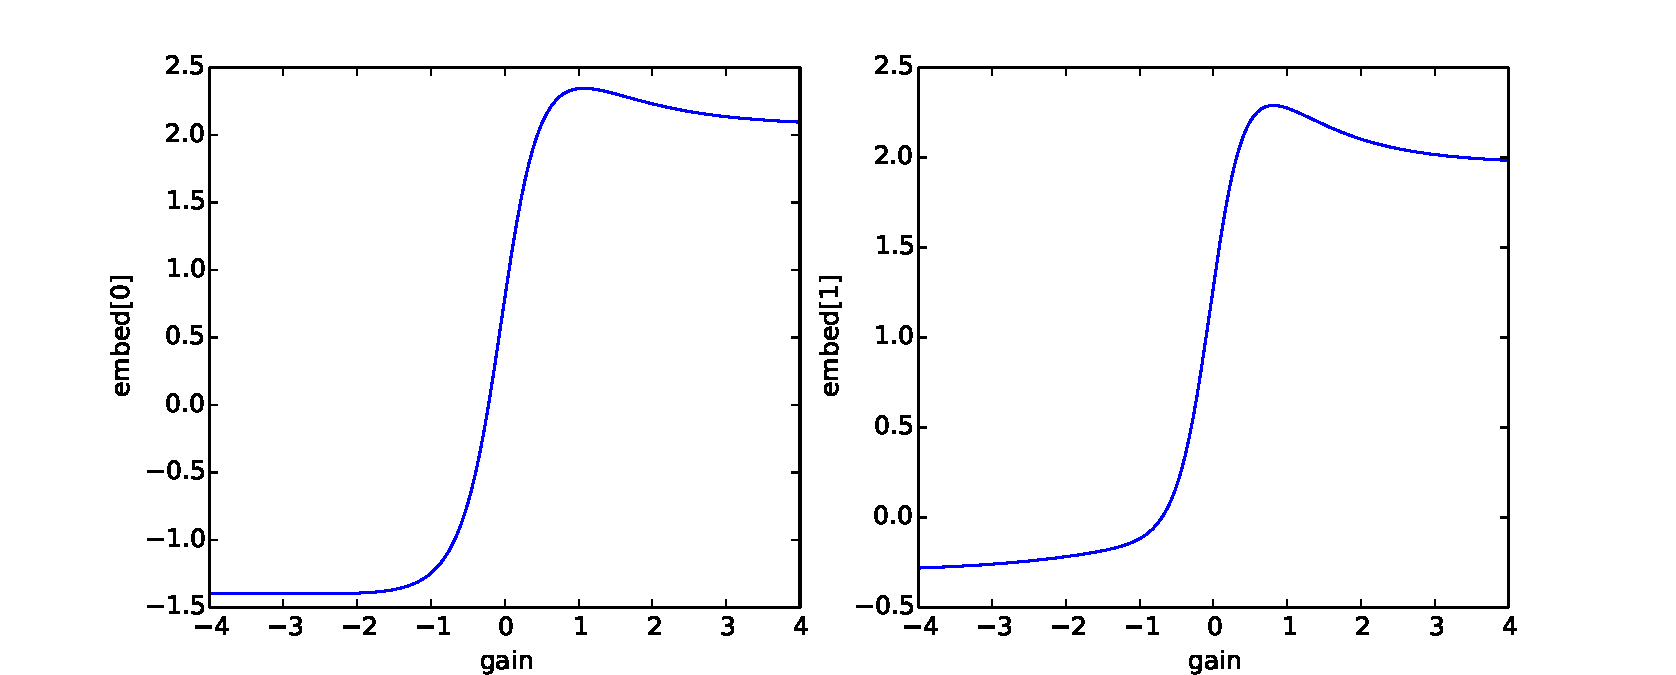
\includegraphics[trim={13.7cm 0 2cm 0}, clip, width=0.4\textwidth]{pointmass_embed_mapping.pdf}
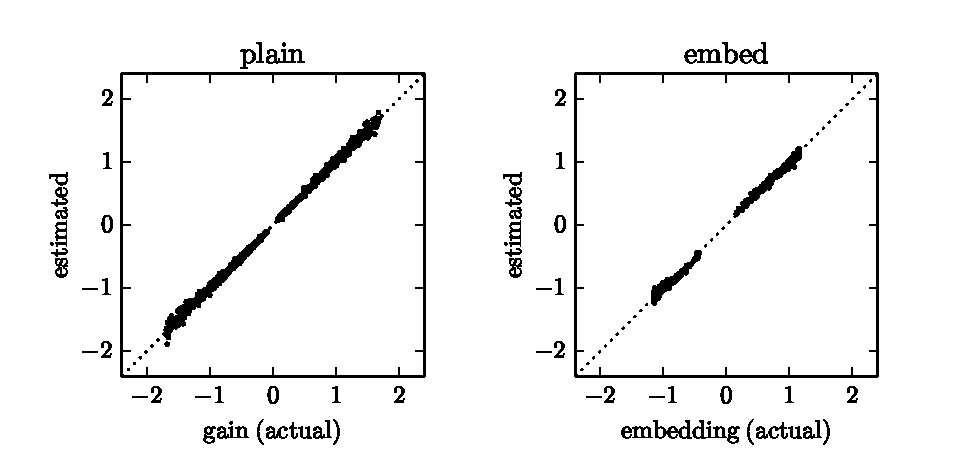
\includegraphics[trim={8.5cm 0 1cm 0}, clip, width=0.36\textwidth]{pointmass_embed_scatter.pdf}
\caption{
\emph{Left}: First dimension of learned mapping $\embedfn$ from gain $g$ to embedding $\latent$.

\emph{Right:} Actual $e(d)$ vs. estimated $\idfn(\tau)$ embedding.

Embedding spreads positive and negative gain to more distant clusters.

Note that optimal policy only depends on sign of $g$.
}
\label{embed-mapping}
\end{figure}
\frametitle{}
\end{frame}


\begin{frame}
\frametitle{Dimensionality reduction: example system}
The learned embedding is capable of performing dimensionality reduction,
making $\idfn$'s estimation task easier.

\begin{block}{Redundant Point-mass system}
\vspace{-.4cm}
\begin{align*}
\text{sysID space}  & : & \cD    &= \good{g, m} \in \pm[0.175, 1.75] &
\text{ (gain factor and \textbf{mass})} \\
\text{dynamics}     & : & \dot p &= v, \quad \dot v = -\epsilon v + \good{\frac{g}{m}} a &
\end{align*}
\end{block}

Note that only the gain-mass \textbf{ratio} affects the dynamics, so it is \textbf{impossible} to estimate both gain and mass from a trajectory.
\end{frame}

\begin{frame}
\frametitle{Dimensionality reduction: results}
\begin{figure}
\centering
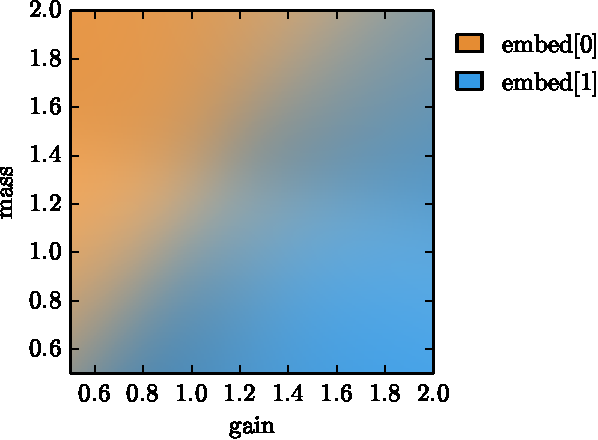
\includegraphics[width=0.5\textwidth]{embed_colors.pdf}
\caption{
Illustration of learned embedding space that disentangles redundant dynamics parameters.
Each gain-mass ratio is mapped to roughly the same embedding value.
Plot restricted to positive gain domain for clarity.
}
\label{fig:embed_colors}
\end{figure}
\end{frame}


\begin{frame}
\frametitle{Half-cheetah environment}

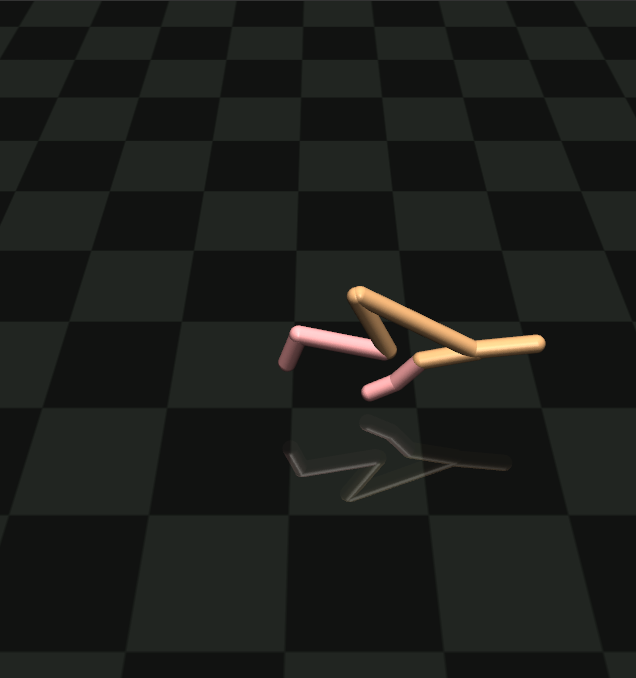
\includegraphics[trim=4cm 3cm 0cm 4cm, clip, width=0.22\textwidth]{cheetah_short.png}\hfill
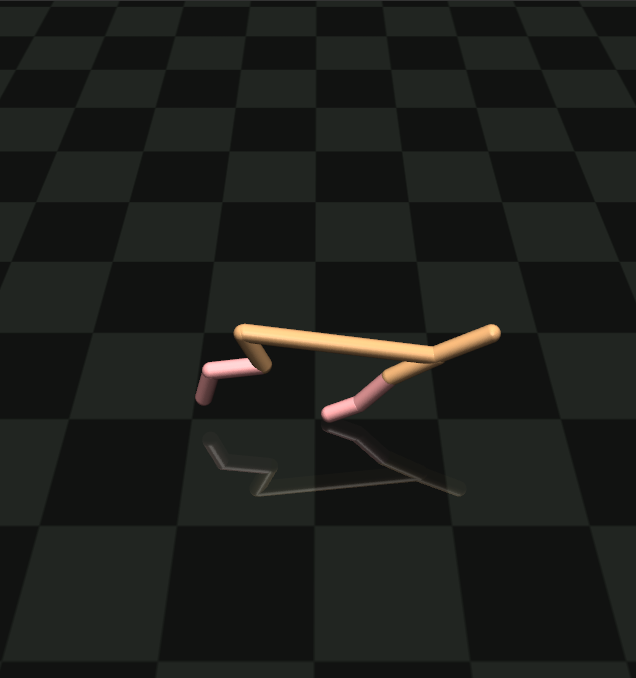
\includegraphics[trim=4cm 3cm 0cm 4cm, clip, width=0.22\textwidth]{cheetah_medium.png}\hfill
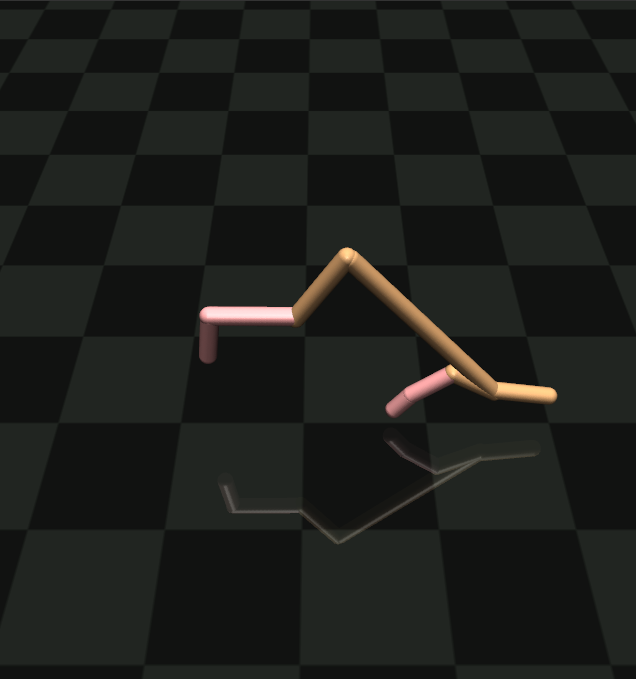
\includegraphics[trim=4cm 3cm 0cm 4cm, clip, width=0.22\textwidth]{cheetah_backleg.png}\hfill
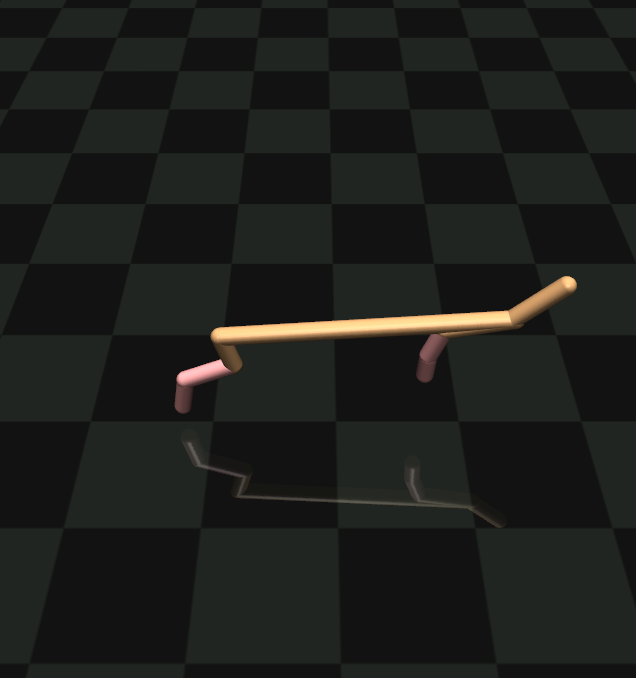
\includegraphics[trim=4cm 3cm 0cm 4cm, clip, width=0.22\textwidth]{cheetah_long.png}

\vspace{0.5cm}
Many parameters randomized:
\begin{itemize}
\item link lengths
\item joint angle ranges
\item rotational damping
\item motor gear ratios
\item friction with ground
\end{itemize}
\end{frame}

\begin{frame}
\frametitle{Half-cheetah results}

\centering
Rewards:

\vspace{0.3cm}

\begin{tabular}{l l l l l l l}
Type & $\alpha_{id}$ & $\mu_{train}$ & $\sigma_{train}$& $\mu_{test}$ & $\sigma_{test}$ & generalization error \\
\hline
\embed{} & 0 & 336.0 & 167.7 & 266.9 & 145.8 & -69.1 \\
\embed{} & \textbf{0.01} & 363.2 & 170.5 & \textbf{288.6} & 145.5 & \textbf{-74.6} \\
\extra{} & 0.0 & 354.9 & 152.2  & 263.7 & 147.4 & -91.2 \\
\extra{} & 0.01 & 370.9 & 149.6 & 274.5 & 141.4 & -96.4 \\
\blind{} & N/A & 266.1 & 156.7 & 244.1 & 140.6 & -22.0
\end{tabular}

\vspace{0.5cm}

\begin{itemize}
\item $\alpha_{id}$: weight of observability term in RL reward.
\item \extra{}: policy without embedding, but extra neural network layers inserted to have same number of parameters as \embed{}.
\item \blind{}: policy with no access to SysID paramters at train or test time (e.g. domain randomization)
\end{itemize}
\end{frame}

\begin{frame}
\frametitle{Implementation notes}
\begin{itemize}
\item RL algorithm: Proximal Policy Optimization (PPO)
\item $\pi$: fully connected neural network, $3 \times 128$ hidden layers, ReLU
\item $\embedfn$: fully connected neural network, $2 \times 74$ hidden layers, ReLU
\item $\idfn$: 1D convolutional neural network, $3$ layers with $64$ filters of width $3$, FC layer of $128$, ReLU
\item Trajectory length $K$ observed by $\idfn$: 16
\end{itemize}

In training, we found stability is improved by including rollouts from several of the sampled dynamics parameters $d \in \cD$ in each optimization step.
\end{frame}

\begin{frame}
\frametitle{Future plans}

\begin{itemize}
\item Our rewards in half-cheetah are substantially below the best achievable by a policy specialized for a single set of parameters $d$.
\item We believe we are bottlenecked by general difficulty of multi-task RL.
\subitem{Currently experimenting with off-policy RL algorithms.}
\item We can get much better results if we train on a small set of systems (e.g. 4 or 8) instead of a dense sampling of $\cD$, but the policy fails to generalize to other systems at test time.
\subitem{Suggests that a good policy for the whole universe must exist.}
\item Different cheetah variations have very different maximum possible rewards -- even a perfect policy would have huge reward variance
\subitem{Is there a way to normalize each environment's rewards?}
\item In our systems, each one action has large long-term consequences. Small errors from bad SysID are still correctible later.
\subitem{SysID might be more important in highly ``feedforward'' settings, e.g. throwing a ball at a target}
\end{itemize}
\end{frame}

\end{document}
